\begin{figure}[H]
    \centering
    % RYSUNEK PRZED KONTRAKCJĄ
    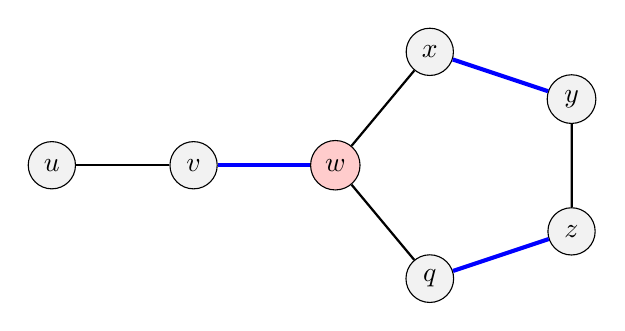
\begin{tikzpicture}[scale=1.2, every node/.style={circle, draw, fill=gray!10, minimum size=0.6cm}]
        % Łodyga
        \node (u) at (0, 0) {$u$};
        \node (v) at (1.5, 0) {$v$};
        % Wierzchołek bazowy (tip)
        \node[fill=red!20] (w) at (3, 0) {$w$}; 

        % Reszta cyklu (kwiatu)
        \node (x) at (4, 1.2) {$x$};
        \node (y) at (5.5, 0.7) {$y$};
        \node (z) at (5.5, -0.7) {$z$};
        \node (q) at (4, -1.2) {$q$};

        % Krawędzie łodygi
        \draw[thick] (u) -- (v);
        \draw[line width=1.5pt, blue] (v) -- (w);

        % Krawędzie cyklu (startujące z bazy w bez dwóch skojarzonych krawędzi z rzędu)
        \draw[thick] (w) -- (x);
        \draw[line width=1.5pt, blue] (x) -- (y);
        \draw[thick] (y) -- (z);
        \draw[line width=1.5pt, blue] (z) -- (q);
        \draw[thick] (q) -- (w);
    \end{tikzpicture}
    \vspace{0.5cm} \\ % Odstęp między rysunkami
    % RYSUNEK PO KONTRAKCJI
    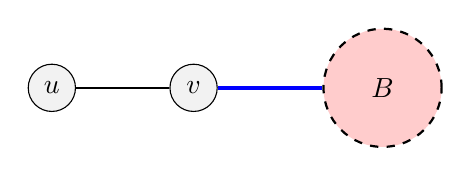
\begin{tikzpicture}[scale=1.2, every node/.style={circle, draw, fill=gray!10, minimum size=0.6cm}]
        \node (u) at (0, 0) {$u$};
        \node (v) at (1.5, 0) {$v$};
        
        % Skontraktowany kwiat
        \node[minimum size=1.5cm, fill=red!20, dashed, thick] (B) at (3.5, 0) {$B$};

        % Łodyga podłączona do super-wierzchołka
        \draw[thick] (u) -- (v);
        \draw[line width=1.5pt, blue] (v) -- (B);
    \end{tikzpicture}
    \caption{U góry: Kwiat oznaczający cykl nieparzystej długości $\{w, x, y, z, q\}$ połączony łodygą z wierzchołkiem wolnym $u$. Wierzchołek $w$ (wyróżniony kolorem) to wierzchołek bazowy (ang. \textit{tip}), w którym spotykają się dwie krawędzie cyklu nienależące do skojarzenia. U dołu: Ten sam graf po operacji kontrakcji kwiatu do pojedynczego super-wierzchołka $B$.}
    \label{rys:kwiat_kontrakcja}
\end{figure}